\documentclass[margin=10pt]{standalone}
\usepackage{color,xcolor}
\usepackage{makecell}
\usepackage{tikz-qtree, tikz}
\usetikzlibrary{arrows.meta,bending}
\usetikzlibrary{calc,trees,positioning,arrows,chains,shapes.geometric,%
    decorations.pathreplacing,decorations.pathmorphing,decorations.markings,shapes,%
    matrix,shapes.symbols,positioning,angles,quotes,patterns}
\usepackage[utf8]{inputenc}

%See https://tex.stackexchange.com/a/29367/1952
\makeatletter
\tikzset{% customization of pattern
        hatch distance/.store in=\hatchdistance,
        hatch distance=5pt,
        hatch thickness/.store in=\hatchthickness,
        hatch thickness=5pt
        }
\pgfdeclarepatternformonly[\hatchdistance,\hatchthickness]{north east hatch}% name
    {\pgfqpoint{-1pt}{-1pt}}% below left
    {\pgfqpoint{\hatchdistance}{\hatchdistance}}% above right
    {\pgfpoint{\hatchdistance-1pt}{\hatchdistance-1pt}}%
    {
        \pgfsetcolor{\tikz@pattern@color}
        \pgfsetlinewidth{\hatchthickness}
        \pgfpathmoveto{\pgfqpoint{0pt}{0pt}}
        \pgfpathlineto{\pgfqpoint{\hatchdistance}{\hatchdistance}}
        \pgfusepath{stroke}
    }
\makeatother

\definecolor{myblue}{HTML}{0072BD}
\definecolor{mygreen}{HTML}{258F1B}
\definecolor{myred}{HTML}{C4000C}

\newcommand{\Ms}{\ensuremath{M_\mathrm{s}}} % Martensite start Temperature
\newcommand{\Mf}{\ensuremath{M_\mathrm{f}}} % Martensite finish Temperature
\newcommand{\As}{\ensuremath{A_\mathrm{s}}} % Austenite start Temperature
\newcommand{\Af}{\ensuremath{A_\mathrm{f}}} % Austenite finish Temperature

% \usetikzlibrary{decorations.pathreplacing,arrows,shapes,positioning,shadows,calc}
% \usetikzlibrary{decorations, decorations.text,backgrounds}
% \tikzset{every picture/.style={font issue=\footnotesize},
%     font issue/.style={execute at begin picture={#1\selectfont}}
% }

\begin{document}
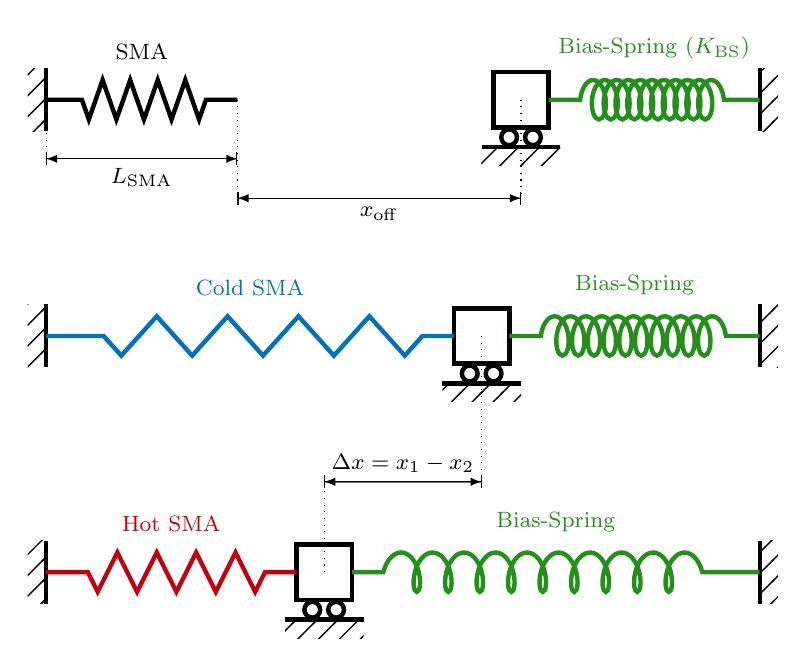
\begin{tikzpicture}[every node/.style={draw,outer sep=0pt,ultra thick,font=\footnotesize}]
\tikzstyle{sma}=[ultra thick,decorate,decoration={zigzag,pre length=4mm,post length=4mm,segment length=5mm, amplitude=2.5mm}]
\tikzstyle{spring}=[ultra thick,decoration={aspect=0.5,pre length=4mm,post length=4mm,segment length=4mm, amplitude=2.5mm,coil},decorate]
\tikzstyle{ground}=[pattern=north east hatch, hatch distance=3mm, hatch thickness=.5pt, fill,draw=none,minimum width=2mm,minimum height=0.1mm]

\tikzstyle{smalong}=[ultra thick,decorate,decoration={zigzag,pre length=4mm,post length=4mm,segment length=9mm, amplitude=2.5mm}]
\tikzstyle{springshort}=[ultra thick,decoration={aspect=0.5,pre length=4mm,post length=4mm,segment length=2mm, amplitude=2.5mm,coil},decorate]

\tikzstyle{smarest}=[ultra thick,decorate,decoration={zigzag,pre length=4mm,post length=4mm,segment length=3.5mm, amplitude=2.5mm}]
\tikzstyle{springrest}=[ultra thick,decoration={aspect=0.5,pre length=4mm,post length=4mm,segment length=1.5mm, amplitude=2.5mm,coil},decorate]

% \tikzstyle{ground}=[fill,pattern=north east lines,draw=none,minimum width=2mm,minimum height=0.1mm]
% \tikzstyle{damper}=[thick,decoration={markings,
%   mark connection node=dmp,
%   mark=at position 0.5 with
%   {
%     \node (dmp) [thick,inner sep=0pt,transform shape,rotate=-90,minimum width=15pt,minimum height=3pt,draw=none] {};
%     \draw [thick] ($(dmp.north east)+(2pt,0)$) -- (dmp.south east) -- (dmp.south west) -- ($(dmp.north west)+(2pt,0)$);
%     \draw [thick] ($(dmp.north)+(0,-5pt)$) -- ($(dmp.north)+(0,5pt)$);
% }
%   }, decorate]
    % SMA - Spring (Hot)
    \node (M) [minimum width=20,minimum height=20] {};
    \node (ground) [ground,anchor=north,yshift=-0.25cm,minimum width=1cm] at (M.south) {};
    \draw[ultra thick] (ground.north east) -- (ground.north west);
    \draw [ultra thick] (M.south west) ++ (0.2cm,-0.125cm) circle (0.1cm)  (M.south east) ++ (-0.2cm,-0.125cm) circle (0.1cm);
    \node (groundL) at (M.east) [ground, xshift=-4cm, rotate=-90, minimum height=0.1mm, minimum width=8mm] {};
    \draw[ultra thick] (groundL.north west) -- (groundL.north east);
    \node (groundR) at (M.west) [ground, xshift=+6cm, rotate=90, minimum height=0.1mm, minimum width=8mm] {};
    \draw[ultra thick] (groundR.north west) -- (groundR.north east);
    \draw[spring, color=mygreen] (M.east) -- node[draw=none, anchor=south, yshift=+4mm] {Bias-Spring} (groundR.north);
    \draw[sma, color=myred] (M.west) -- node[draw=none, anchor=south, yshift=+4mm] {Hot SMA} (groundL.north);

    % Cold SMA Bias Spring
    \begin{scope}[yshift=3cm]
        \node (Mc) [minimum width=20,minimum height=20] at (2,0){};
        \node (ground) [ground,anchor=north,yshift=-0.25cm,minimum width=1cm] at (Mc.south) {};
        \draw[ultra thick] (ground.north east) -- (ground.north west);
        \draw [ultra thick] (Mc.south west) ++ (0.2cm,-0.125cm) circle (0.1cm)  (Mc.south east) ++ (-0.2cm,-0.125cm) circle (0.1cm);

        \node (groundL) at (Mc.east) [ground, xshift=-6cm, rotate=-90, minimum height=0.1mm, minimum width=8mm] {};
        \draw[ultra thick] (groundL.north west) -- (groundL.north east);
        \node (groundR) at (Mc.west) [ground, xshift=+4cm, rotate=90, minimum height=0.1mm, minimum width=8mm] {};
        \draw[ultra thick] (groundR.north west) -- (groundR.north east);

        \draw[springshort, color=mygreen] (Mc.east) -- node[draw=none, anchor=south, yshift=+4mm] {Bias-Spring} (groundR.north);
        \draw[smalong, color=myblue] (Mc.west) -- node[draw=none, anchor=south, yshift=+4mm] {Cold SMA} (groundL.north);
    \end{scope}

    \node[yshift=+1.5cm, draw=none] (xc) at (M.south) {};
    \node[yshift=-1.5cm, draw=none] (xh) at (Mc.south) {};
    \draw[|-|] (xc.center)-- node[above, draw=none] {$\Delta x = x_1 - x_2$} (xh.center);
    \draw[latex-latex] (xc.center)-- (xh.center);
    \draw[dotted] (M.center)--(xc.center);
    \draw[dotted] (Mc.center)--(xh.center);

    % Disconnected SMA Bias Spring
    \begin{scope}[yshift=6cm]
        \node (Mr) [minimum width=20,minimum height=20] at (2.5,0){};
        \node (groundRR) [ground,anchor=north,yshift=-0.25cm,minimum width=1cm] at (Mr.south) {};
        \draw[ultra thick] (groundRR.north east) -- (groundRR.north west);
        \draw [ultra thick] (Mr.south west) ++ (0.2cm,-0.125cm) circle (0.1cm)  (Mr.south east) ++ (-0.2cm,-0.125cm) circle (0.1cm);

        \node (groundLR) at (Mr.east) [ground, xshift=-6.5cm, rotate=-90, minimum height=0.1mm, minimum width=8mm] {};
        \draw[ultra thick] (groundLR.north west) -- (groundLR.north east);
        \node (groundRR) at (Mr.west) [ground, xshift=+3.5cm, rotate=90, minimum height=0.1mm, minimum width=8mm] {};
        \draw[ultra thick] (groundRR.north west) -- (groundRR.north east);

        \draw[springrest, color=mygreen] (Mr.east) -- node[draw=none, anchor=south, yshift=+4mm] {Bias-Spring $(K_\mathrm{BS})$} (groundRR.north);
        \draw[smarest, color=black] ($(Mr.west)-(3.25,0)$) -- node[draw=none, anchor=south, yshift=+4mm] {SMA} (groundLR.north);
    \end{scope}

    % \node[yshift=-1.25cm, draw=none] (xcr) at (groundLR.north) {}; % Start of resting SMA
    \node[yshift=-1.25cm, draw=none] (xcr) at ($(Mr.west)-(3.25,0)$) {};
    \node[yshift=-1.25cm, draw=none] (xhr) at (Mr.center) {};
    \draw[|-|] (xcr.center)-- node[below, draw=none] {$x_\mathrm{off}$} (xhr.center);
    \draw[latex-latex] (xcr.center)-- (xhr.center);
    % \draw[dotted] (groundLR.north)--(xcr.center); % Start of resting SMA
    \draw[dotted] ($(Mr.west)-(3.25,0)$)--(xcr.center);
    \draw[dotted] (Mr.center)--(xhr.center);

    \node[yshift=-0.75cm, draw=none] (xcr) at (groundLR.north) {};
    \node[yshift=-0.75cm, draw=none] (xhr) at ($(Mr.west)-(3.25,0)$) {};
    \draw[|-|] (xcr.center)-- node[below, draw=none] {$L_\mathrm{SMA}$} (xhr.center);
    \draw[latex-latex] (xcr.center)-- (xhr.center);
    \draw[dotted] (groundLR.north)--(xcr.center);
    \draw[dotted] ($(Mr.west)-(3.25,0)$)--(xhr.center);

\end{tikzpicture}
\end{document}
